\documentclass{article}
\usepackage[utf8]{inputenc}
\usepackage{graphicx,fancyhdr,amsmath,amssymb,amsthm,subfig,url,hyperref,enumerate}

% For payoff matrices
\usepackage{multirow,enumerate,array,float}
\usepackage[margin=1in]{geometry}

% For figures
\usepackage{graphicx}
\graphicspath{ {./figures/} }

\begin{document}
\title{Improving healthcare outcomes and cost through analysis and design of provider incentives}
\author{Keyan Pishdadian\\University of Washington\\\texttt{keyanp@cs.washington.edu}}
\date{March 2020}

\maketitle

\begin{abstract}
Provider decision making plays a critical role in patient outcomes and national healthcare spending. Creating robust incentive structures to underlie provider decision making are vital to ensuring the delivery of high quality care and adequately managed costs. Despite this these incentive structures are poorly designed both financially and from a provider risk perspective. In this paper I analyze the inefficiencies and sub-optimal equilibria that result from the use of classic incentive systems, then extend recent ideas to propose a hybrid incentive structure that increases provider profits, improves patient outcomes, and reduces wasteful spending.
\end{abstract}

\section{Introduction}
Healthcare is a socially and economically important aspect of the modern United States. Roughly 1/6th of US consumer spending \cite{econharvard} and ${\sim}48$\% of federal spending \cite{federalspend} goes towards some form of healthcare and the success, efficiency, and outcomes of this market reflect directly on the viability and happiness of American citizens and the US economy. The decision making of physicians plays a integral role in this system, with roughly 80\% of all expenditure being a result of physicians' decisions \cite{trust}. One becomes concerned with this control when comparing US healthcare expenditure to other developed countries (Fig. \ref{fig:usspend}), just why is expenditure so much higher in the US without better outcomes \cite{acoecon}? At the root of the issue is that the healthcare market is unlike other normal markets where there is a buyer and a seller, with the buyer fully knowing what it is they want and having transparency into the price being offered by the seller \cite{msdt}. Rather, in this market there are many agents interacting directly or indirectly within a single healthcare transaction.

This results in a complex web of interdependencies between the agents (Fig. \ref{fig:agentdep}) which significantly complicates construction of effective incentive structures. Additionally the patient has little control in their outcomes aside from selecting a provider. In fact, the patient-provider relationship is a clear example of a \emph{principle-agent problem} \cite{principle} where the provider (the ``agent") must make diagnosis and care decisions that impact the patient (the ``principle"), but the provider/agent is motivated to act in their own best interests and not in the best interest of the patient/principle \cite{msdt}. Simultaneously, the provider is engaged in a game with other providers that closely resembles a ``prisoners' dilemmas", ultimately the decision making of any one provider has externalities on the health of the entire patient population, with a future decrease in overall health leading to an increase in the required volume of care to sustain proper health \cite{blended}.

In this paper I present each of the prevailing provider incentive structures, examine their benefits and inefficiencies, then use an adapted simplified model to formalize the resulting equilibria reached in each system. I briefly review the prisoners' dilemma model as a framework for analyzing provider decision making. I then extend recent ideas from Accountable Care Organizations (ACOs) to propose and analyze a hybrid incentive structure that increases provider profits and improves patient outcomes.

\begin{figure}[H]
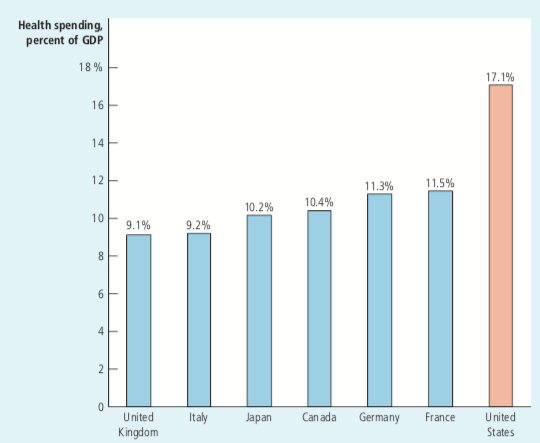
\includegraphics[height=7cm]{usspend}
\centering
\caption{US healthcare expenditure is significantly higher than that of other developed countries \cite{econharvard}.}
\label{fig:usspend}
\end{figure}

\section{Setup}

\subsection{Agents}
To begin analysis of the current state of healthcare it is required to examine who is involved and what they are optimizing for. Because the scope of this system is large, I limit the number of agents and make some assumptions about their motivations to simplify the future model. An overview of the agents is provided in Fig. \ref{fig:agentdep}, and they are summarized below.

\paragraph{Payer:}The payer can be thought of as both an individual patient or alternatively some entity which is responsible for paying for services rendered to others it is responsible for. Generally the latter case would be an employer or government which is providing health insurance to others at cost. While insurance companies are also considered a payer, they are outside the scope of this work. Note that oftentimes there are multiple payers involved in a single healthcare transaction, although here it is assumed that they are all aligned with respect to their goals.

Ultimately the payer seeks to minimize cost, while maximizing quality of service. In the case of a patient the desire to maximize quality of service is self-explanatory, and in the case of an employer/government the intention is that high quality of service will mean higher general health and less future demand for healthcare, which drives down cost.

\paragraph{Provider:}These are any individuals rendering services for payers. Generally providers can be thought of as physicians. Providers seek to maximize revenue\footnote{In order to simplify the model I ignore any altruistic behavior and moral incentives that I imagine (and hope) are present to some extent.} to themselves and also minimizing financial and professional risk (e.g. malpractice lawsuits).

The provider is the central agent in this model because as mentioned previously, their decisions account for ${\sim}80$\% of healthcare spending \cite{trust}. Importantly the payoff of any one provider is influenced by the collective behavior of other providers in the system. A provider may choose to render low quality service and thus negatively affect the health of a patient and through this they can impart externalities on other providers, whether those are negative or positive depends on the payment system.

\paragraph{Hospital:}A hospital manages the compensation of providers and negotiates with payers to determine costs. Hospitals seek to maximize revenue by minimizing cost. Traditionally this also means maximizing volume of services rendered while minimizing quality of those services, but this fact can vary with the compensation structure being used. This paper does not focus on the actions of a hospital other than presenting them as a possible organizer and controller of providers given that the hospital is designing the provider compensation system.

\begin{figure}[H]
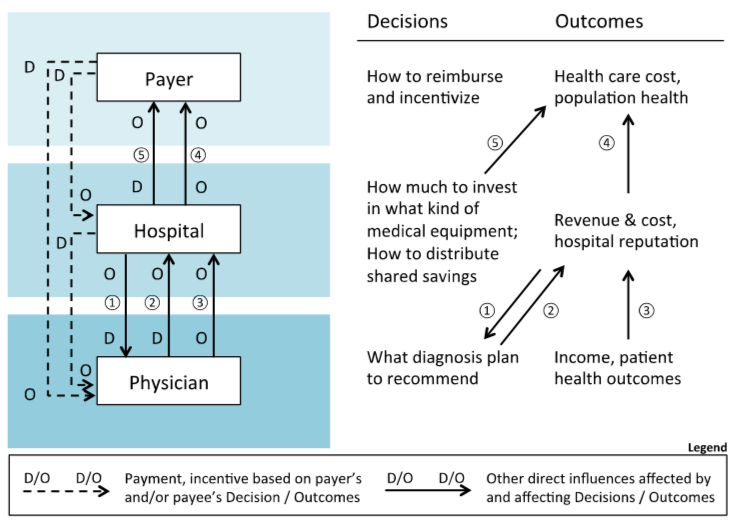
\includegraphics[height=7cm]{agentdep}
\centering
\caption{Agent interdependence diagram which shows the complex network of interactions between payers, providers (Physician), and hospitals. In this work I focus on controlling the provider decision making process (relations $1$ and $2$) as a means of improving payer health outcomes and cost (relation $4$) \cite{msdt}.}
\label{fig:agentdep}
\end{figure}

\subsection{Incentive Modeling}
In order to create a framework to analyze provider actions and payoffs in the existing and proposed payment models, the following set of notation is introduced (adapted from \cite{trust}\cite{blended}) to represent the different variables involved:

\begin{itemize}
    \item \textbf{V} - Volume of services. An independent variable that is a result of provider decisions.
    \item \textbf{Q} - Quality of services. An independent variable that is a result of provider decisions.
    \item \textbf{C} - Capitation rate (explained in \ref{sec:capitation}). Dependent on the payment model.
    \item \textbf{B} - Bonus incentive. Dependent on the payment model and provider decisions.
    \item \textbf{T} - Trust score. Dependent on provider decisions.
\end{itemize}

In this model the provider is able to control $V$ and $Q$, by either performing a low or high volume of service ($V_{low}$, $V_{high}$), and either low or high quality service ($Q_{low}$, $Q_{high}$), the pair of provider actions in a model is represented as $(V, Q)$. Capitation rate is dependent on the payment model being used. In general $C \in [0, 5]$, with $0$ being no use of capitation and $10$ being a pure capitation model. Externalities are also determined by provider quality decision so we the notation $E_{Q_{high}}$ and $E_{Q_{low}}$ are used to represent the resulting externalities caused by a decision to give high and low quality service, respectively. In some payment models $E_{Q_{high}} \in \mathbb{R}^+$, while in others $E_{Q_{high}} \in \mathbb{R}^-$, but one can imagine that an ideal system is one that incentivizes providing high quality service by ensuring that results in positive externalities on other providers.

The \emph{bonus incentive} ($B$) and \emph{trust score} ($T$) variables are new concepts that I leverage to sway provider decision making by rewarding desirable provider behavior. The bonus is adapted from ideas presented in ACOs (see \ref{sec:aco}), this value is computed based on past provider behavior over a defined interval and retroactively rewards responsible actions. The trust score is a form of a reputation system \cite{tim} that controls 

//TODO

\section{Existing Payment Models}
In this section I review the two major incentive structures used for provider payment, \textbf{fee-for-service} and \textbf{capitation}. Discussion of the issues with each structure gives motivation to understanding the novel payment structure used by ACOs.

\subsection{Fee-for-service}
This model is most familiar to anyone who has interfaced with US healthcare. Here a provider is payed for each service rendered (e.g. surgery, office visit). Hence the payment to the provider is a direct function of the volume of services provided. Of course a clear conflict of interest is presented, providers are incentivized to provide a high volume of low quality and high cost services, regardless of need. Aside from ethical considerations, the outcome of the patient has no bearing on the payoff of the provider. This observation is not surprising given the principle-agent backdrop coloring this relationship, and this has been documented an expectation of patients and other providers alike \cite{econharvard}\cite{overtreat}.

So what does this method get right? That same indifference to cost that begets high volume service may also allows access to expensive services that may give good results but have low probability of success. When providers do not fear increased spending then they are free to explore new treatment methods, equipment, medications, and procedures.

Using the incentive model the payoff under this payment system as is represented as:
\begin{equation}
    \text{payoff} = V + Q + E
\end{equation}

Where it can assume high quality services actually result in an increase of collective patient health which causes \emph{negative} externalities for other providers, who would now have fewer patients to treat and thus less service volume to bill for, i.e. $E_{Q_{high}} \in \mathbb{R}^-$.

//TODO
Similar analysis performed in \cite{blended} as to the prisoners' dilemma presented in 

\subsection{Capitation} \label{sec:capitation}
The capitation model is on the other end of the spectrum relative to fee-for-service models. Here a provider is paid a fixed sum for an agreed upon length of time for each patient that they oversee the health of. There are a wide range of methods used to compute capitation fees and payments structures that are outside the scope of this paper and discussed elsewhere, e.g. \cite{capfees}. Overall the principle is that providers want to reduce the number of services rendered and keep patients healthy so that they do no exceed the negotiated rate of payment per patient. Because any amount of spending beyond the negotiated capitation rate is entirely the responsibility of the provider/hospital, this model shifts significant risk to the provider to keep costs low, but has potential for greater financial payoff if the total cost of services rendered is significantly below the capitation fee.

Supporters of this model cite that it succeeds in reducing provider incentives to provide high volume services that are driven more by billing ability than by patient need \cite{blended}. However, there is fear that this design results instead in a low volume of low quality services. In fact it is this model that causes a prisoners' dilemma to arise between providers. Collectively all providers are better off if the health of the patient population in aggregate is good, as this means those patients will impose lower costs on each provider, but each provider's \emph{best response} strategy when making a care decision is ultimately to still provide low volume low quality care and free-ride on any provider that might be providing high volume high quality care. This point is formalized further in \textbf{Modeling Incentives}.

Using the incentive model the payoff under this payment system as is represented as:
\begin{equation}
    \text{payoff} = V + Q + E + C
\end{equation}

Where it can assume high quality services results in an increase of collective patient health which causes \emph{positive} externalities for other providers, who would now have fewer patients to treat and thus reduce their future costs, i.e. $E_{Q_{high}} \in \mathbb{R}^+$.

\subsection{Accountable Care Organizations (ACOs)} \label{sec:aco}
ACOs were introduced as an attempt to mitigate some of the issues with both of the aforementioned payment structures. Formally enacted as part of the Patient Protection and Affordable Care Act of 2010, over 10.5 million Medicare patients have been assigned to ACOs over recent years and there are data to support that there has been federal significant savings using the system \cite{acos}.

An ACO is a group of providers who choose to join that organization and together treat Medicare patients. The Centers for Medicare \& Medicare (CMS) is a federal agency which sets an maximum expenditure benchmark for that ACO based on prior Medicare expenses and cost forecasting. Together providers in the ACO render services using a standard fee-for-service payment model, but if the total spending during a pre-defined time interval is below the expenditure benchmark then the ACO receives up to ${\sim}50$\% of the savings as a cash incentive bonus, depending on an additional \emph{quality score} \cite{acos}. The exact computation of earnings depends on the negotiated ACO incentive structure and the quality score which is determined by evaluating performance on annually set CMS benchmarks, e.g. percentage of patients provided with preventative screening and influenza vaccination (detailed quality benchmarks can be found on the CMS website \cite{cms}). Accordingly a representative formula for savings bonus calculation would be (adapted from \cite{acos}):

\begin{equation}
    \text{Bonus} = \max (0, 0.5 * (\text{Spending Benchmark} - \text{Actual Spending}) * \text{Quality Score})
\end{equation}

This incentive structure has some nice intuitive properties. The spending benchmark and associated savings bonus escape incentives to overspend seen in the fee-for-service model, while the use of a quality score avoids the natural best response of underspending observed in the capitation model and which would likely occur here as well. And yet ACOs are not the final answer.

//TODO
\begin{itemize}
    \item Financial side effects - hospitals use sub-optimal drugs that don't apply to the benchmark calculation \cite{acoethics}.
    \item Bonus sharing - hospitals control the savings bonus, how to distribute it is complicated and prone to hospitals acting in their own self-interest \cite{inflation}. Additionally there is no aspect of the design that rewards good actors and penalizes bad actors. ACOs are left to their own decisions on how to appropriately compensate providers that have positive externalities on the system.
    \item Increase in power - the ACO system leads itself to large groups of providers/hospitals organizing and having increased market share. With this size comes the ability to control the market and raise prices for payers. This may even entirely offset any expected savings \cite{acoecon}.
    \item Complexity - //TODO
\end{itemize}

Using the incentive model the payoff under this payment system as is represented as:
\begin{equation}
    \text{payoff} = V + Q + E + B
\end{equation}

// TODO
% Where we can assume high quality services results in an increase of collective patient health which causes \emph{positive} externalities for other providers, who would now have fewer patients to treat and thus reduce their future costs, i.e. $E_{Q_{high}} \in \mathbb{R}^+$.

\subsection*{Prisoners'/Providers' Dilemma}
For a thorough treatment of the prisoners' dilemma, refer to any number of game theory texts, e.g. \cite{networks}

\begin{table}[H]
\centering
  \setlength{\extrarowheight}{2pt}
  \begin{tabular}{*{4}{c|}}
    \multicolumn{2}{c}{} & \multicolumn{2}{c}{Prisioner II}\\\cline{3-4}
    \multicolumn{1}{c}{} &  & $S$  & $C$ \\\cline{2-4}
    \multirow{2}*{Prisioner I}  & $S$ & $(2,2)$ & $(12,1)$ \\\cline{2-4}
    & $C$ & $(1,12)$ & $(12,12)$ \\\cline{2-4}
  \end{tabular}
\caption{Payoff matrix zero-sum number calling game.}
\end{table}

\section{Hybrid Approach}

\section{Conclusions}

%--------------------------------- Tables ----------------------------------


%--------------------------------- Figures ----------------------------------

\begin{figure}
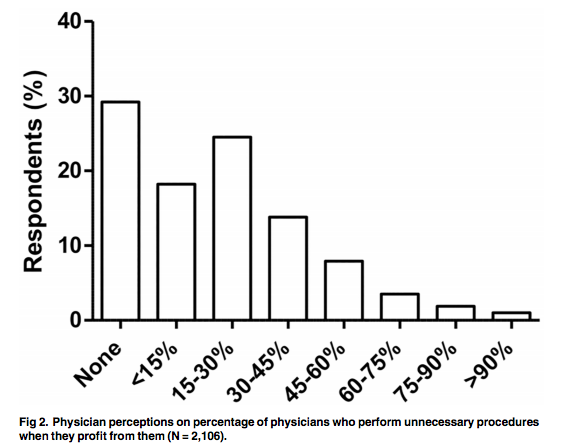
\includegraphics[height=7cm]{overtreat}
\centering
\caption{Provider responses when surveyed and asked what percentage of other physicians they think perform uneeded procedures financial gain \cite{overtreat}.}
\label{fig:overtreat}
\end{figure}

%--------------------------------- Bibliography ----------------------------------

\clearpage

\begin{thebibliography}{8}

\bibitem{federalspend}
The True Cost of Health Care: An Analysis of Americans’ Total Health Care Spend. https://bit.ly/39wbFzi

\bibitem{econharvard}
Mankiw NG. (2017) The Economics of Healthcare.

%6
\bibitem{trust}
Djulbegovic, Benjamin \& Hozo, Iztok \& Ioannidis, John. (2014). Modern health care as a game theory problem. European Journal of Clinical Investigation. 45. 10.1111/eci.12380

\bibitem{overtreat}
Lyu H, Xu T, Brotman D, Mayer-Blackwell B, Cooper M, Daniel M, et al. (2017). Overtreatment in the United States. PLoS ONE 12(9): e0181970. https://doi.org/10.1371/journal.pone.0181970

%4
\bibitem{blended}
DeVoe, J. E., \& Stenger, R. (2013). Aligning provider incentives to improve primary healthcare delivery in the United States. OA family medicine, 1(1), 7. doi:10.13172/2052-8922-1-1-958

%5
\bibitem{msdt}
Zhang, H., Wernz, C. \& Slonim, A.D. (2016). Aligning incentives in health care: a multiscale decision theory approach. EURO J Decis Process 4, 219–244. https://doi.org/10.1007/s40070-015-0051-3

\bibitem{principle}
Eisenhardt, K. (1989). Agency Theory: An Assessment and Review. The Academy of Management Review, 14(1), 57-74. www.jstor.org/stable/258191

\bibitem{networks}
David, E., Kleinberg, J. (2010). Networks, Crowds, and Markets: Reasoning About a Highly Connected World. Cambridge University Press, USA. https://www.cs.cornell.edu/home/kleinber/networks-book/

\bibitem{acos}
Redding, K. (2018). Participation and Performance in Accountable Care Organizations, Doctoral Disertation.

\bibitem{capfees}
Iezzoni, Lisa I. et al. (1998). Paying More Fairly for Medicare Capitated Care. New England Journal of Medicine. https://doi.org/10.1056/NEJM199812243392613

\bibitem{acoecon}
Blackstone, E. A., \& Fuhr, J. P., Jr (2016). The Economics of Medicare Accountable Care Organizations. American health \& drug benefits, 9(1), 11–19.

\bibitem{cms}
https://www.cms.gov/Medicare/Medicare-Fee-for-Service-Payment/sharedsavingsprogram/Downloads\-/2018-and-2019-quality-benchmarks-guidance.pdf

% 1
% Cite as complicated approach by modifying how hospitals bill for services
\bibitem{inflation}
Agee, M.D., Gates, Z. (2013). Lessons from Game Theory about Healthcare System Price Inflation. Appl Health Econ Health Policy 11, 45–51. https://doi.org/10.1007/s40258-012-0003-z

\bibitem{acoethics}
Virtual Mentor. 2013;15(2):156-161. doi: 10.1001/virtualmentor.2013.15.2.pfor1-1302.

\bibitem{tim}
Roughgarden, T. (2016). Asymmetric Information and Reputation Systems. http://timroughgarden.org/f16/l/l12.pdf

\end{thebibliography}

%-------------------------------------------------------------------

\end{document}
